\documentclass[11pt,a4paper]{article}
\usepackage[margin=27mm]{geometry}
\usepackage{amsmath,amssymb,amsthm,mathtools}
\usepackage{booktabs}
\usepackage{tikz}
\usetikzlibrary{arrows.meta,calc,positioning,angles,quotes}
\usepackage[hidelinks]{hyperref}
\usepackage{microtype}
\usepackage{fancyvrb}
\setlength{\emergencystretch}{3em}

\newtheorem{theorem}{Theorem}[section]
\newtheorem{proposition}[theorem]{Proposition}
\newtheorem{lemma}[theorem]{Lemma}
\newtheorem{definition}[theorem]{Definition}
\newtheorem{remark}[theorem]{Remark}

\newcommand{\QQ}{\mathbb{Q}}
\newcommand{\KK}{K}
\newcommand{\R}{\mathbb{R}}
\newcommand{\Res}{\operatorname{Res}}
\newcommand{\Norm}{\operatorname{Norm}}
\newcommand{\crit}{R_{\mathrm{crit}}}
\newcommand{\Rzero}{R_0}

\title{Two Equivalent Algebraic Definitions of the Critical Radius\\
for a Ten-Circle Contact Configuration}
\author{Computer-assisted exact-arithmetic note}
\date{October 2026}

\begin{document}
\maketitle

\begin{abstract}
We compare two definitions of the same radius for a fixed contact
configuration of ten circles with radii $r_i=\sqrt{i}$.  The first definition,
$R_0$, is algebraic: it is the isolated real root of a degree--1792 rational
norm polynomial obtained from contact elimination.  The second definition,
$R_{\mathrm{crit}}$, is geometric: it is the unique $R$-coordinate of the
solution of two angular closure equations $A(t,R)=B(t,R)=2\pi$.  We explain
the exact implication from the angular equations to the eliminant and hence
the identification $R_{\mathrm{crit}}=R_0$, conditional on the explicitly
stated certificate bridge.  This note does not prove global
optimality over all contact configurations.
\end{abstract}

\tableofcontents

\section{Introduction}

The purpose of this note is deliberately narrow.  We do not claim that the
selected contact configuration is globally optimal among all configurations
of ten unequal circles.  Instead, we prove that two independently useful
definitions of its radius describe the same real number:
\[
  \boxed{R_{\mathrm{crit}}=R_0}.
\]
The first definition is convenient for exact algebraic computation, while the
second is convenient for geometric angle-barrier arguments.

The selected contacts are
\[
\begin{gathered}
(10,5),(10,7),(10,6),(5,7),\\
(7,9),(9,2),(2,8),(8,6).
\end{gathered}
\]

\begin{remark}
The equality proved here is an identity between two definitions of a fixed
contact-configuration radius.  It is not a proof of $R^*=R_0$ for the full
packing problem; that is a separate global-coverage question.
\end{remark}

\section{Contact configuration and notation}

Let
\[
 r_i=\sqrt{i},\qquad i=1,\ldots,10,
\]
and let $R$ be the containing-circle radius.  For a wall-contacting circle,
write
\[
 t_i=R-r_i.
\]
The distinguished cyclic order is
\[
 10\longrightarrow5\longrightarrow7\longrightarrow9
 \longrightarrow2\longrightarrow8\longrightarrow6\longrightarrow10.
\]

\begin{figure}[ht]
\centering
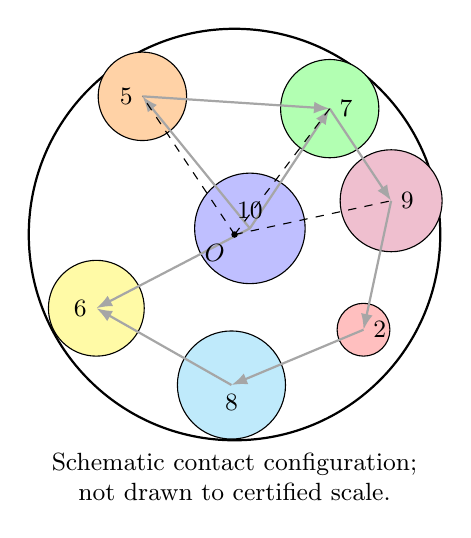
\begin{tikzpicture}[scale=0.78, every node/.style={font=\small}]
  \draw[thick] (0,0) circle (3.35);
  \coordinate (O) at (0,0);
  \coordinate (c10) at (0.25,0.10);
  \coordinate (c5) at (-1.50,2.25);
  \coordinate (c7) at (1.55,2.05);
  \coordinate (c9) at (2.55,0.55);
  \coordinate (c2) at (2.10,-1.55);
  \coordinate (c8) at (-0.05,-2.45);
  \coordinate (c6) at (-2.25,-1.20);
  \foreach \p/\rr/\col in {c10/0.90/blue!25,c5/0.72/orange!35,c7/0.80/green!30,c9/0.83/purple!25,c2/0.43/red!25,c8/0.88/cyan!25,c6/0.78/yellow!35}{
    \draw[black, fill=\col] (\p) circle (\rr);
  }
  \foreach \a/\b in {c10/c5,c10/c7,c10/c6,c5/c7,c7/c9,c9/c2,c2/c8,c8/c6}{
    \draw[-{Latex[length=2mm]}, thick, gray!70] (\a)--(\b);
  }
  \foreach \p/\lab/\pos in {c10/10/above,c5/5/left,c7/7/right,c9/9/right,c2/2/right,c8/8/below,c6/6/left}{
    \node[\pos] at (\p) {$\lab$};
  }
  \fill (O) circle (1.5pt) node[below left] {$O$};
  \draw[dashed] (O)--(c5);
  \draw[dashed] (O)--(c7);
  \draw[dashed] (O)--(c9);
  \node[align=center] at (0,-3.95) {Schematic contact configuration;\\not drawn to certified scale.};
\end{tikzpicture}
\caption{The selected seven-circle core and its contact edges. The three
remaining circles are rattlers for the displayed witness only; they are not
used in the algebraic elimination.}
\label{fig:contact}
\end{figure}

\section{Contact geometry}

For two circles with center radii $s_i,s_j>0$, define the necessary small
angle
\[
 \phi_{ij}(s_i,s_j)=arccos\left(
 \frac{s_i^2+s_j^2-(r_i+r_j)^2}{2s_is_j}\right).
\]
For the six wall circles and circle 10 put
\[
 \alpha_i(t,R)=\phi_{10,i}(t,R-r_i),
 \qquad
 \beta_{ij}(R)=\phi_{ij}(R-r_i,R-r_j).
\]

The following diagram shows the two angle sums.  The second path omits the
term involving circle 5; it is a second necessary angular closure condition,
not a claim that circle 5 is removed from the packing.

\begin{figure}[ht]
\centering
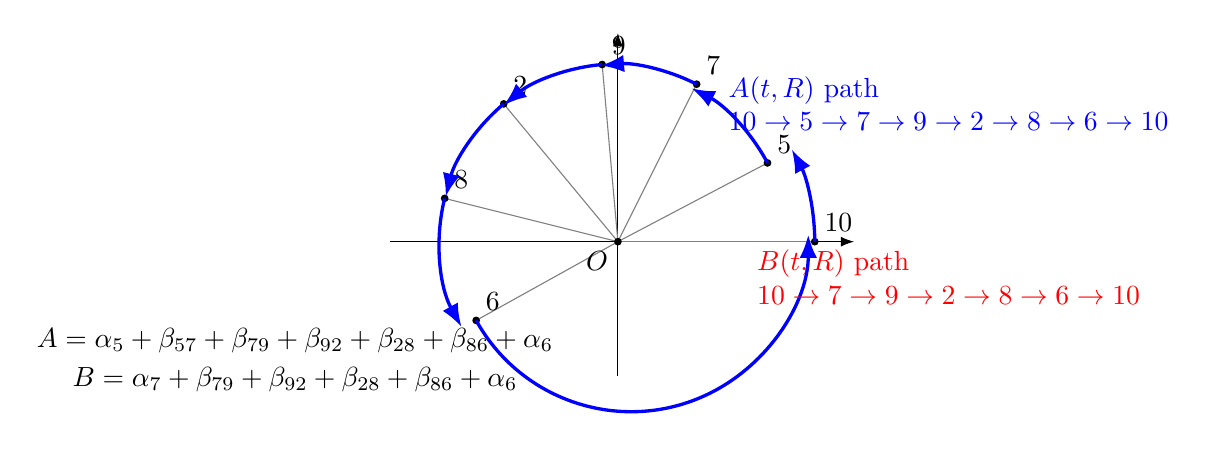
\begin{tikzpicture}[x=1cm,y=1cm,>=Latex]
  \coordinate (O) at (0,0);
  \coordinate (p10) at (2.5,0);
  \coordinate (p5) at (1.9,1.0);
  \coordinate (p7) at (1.0,2.0);
  \coordinate (p9) at (-0.2,2.25);
  \coordinate (p2) at (-1.45,1.75);
  \coordinate (p8) at (-2.2,0.55);
  \coordinate (p6) at (-1.8,-1.0);
  \draw[->] (-2.9,0)--(3.0,0);
  \draw[->] (0,-1.7)--(0,2.65);
  \foreach \p/\lab in {p10/10,p5/5,p7/7,p9/9,p2/2,p8/8,p6/6}{
    \draw[gray] (O)--(\p);
    \fill (\p) circle (1.4pt) node[above right] {$\lab$};
  }
  \fill (O) circle (1.4pt) node[below left] {$O$};
  \draw[very thick, blue, ->] (p10) arc (0:28:2.5);
  \draw[very thick, blue, ->] (p5) arc (28:63:2.25);
  \draw[very thick, blue, ->] (p7) arc (63:95:2.25);
  \draw[very thick, blue, ->] (p9) arc (95:130:2.25);
  \draw[very thick, blue, ->] (p2) arc (130:166:2.25);
  \draw[very thick, blue, ->] (p8) arc (166:209:2.25);
  \draw[very thick, blue, ->] (p6) arc (209:360:2.25);
  \node[blue,align=left] at (4.2,1.75) {$A(t,R)$ path\\
  $10\to5\to7\to9\to2\to8\to6\to10$};
  \node[red,align=left] at (4.2,-0.45) {$B(t,R)$ path\\
  $10\to7\to9\to2\to8\to6\to10$};
  \node[align=left] at (-4.1,-1.25) {$A=\alpha_5+\beta_{57}+\beta_{79}+\beta_{92}+\beta_{28}+\beta_{86}+\alpha_6$};
  \node[align=left] at (-4.1,-1.75) {$B=\alpha_7+\beta_{79}+\beta_{92}+\beta_{28}+\beta_{86}+\alpha_6$};
\end{tikzpicture}
\caption{Schematic angular decomposition. The blue and red paths share the
chain from 7 through 6; their difference is the rigid-triangle relation.}
\label{fig:angles}
\end{figure}

\section{The geometric definition of $R_{\mathrm{crit}}$}

Define
\[
\begin{aligned}
A(t,R)&=\alpha_5+\beta_{57}+\beta_{79}+\beta_{92}+\beta_{28}+\beta_{86}+\alpha_6,\\
B(t,R)&=\alpha_7+\beta_{79}+\beta_{92}+\beta_{28}+\beta_{86}+\alpha_6.
\end{aligned}
\]

\begin{definition}
Let $(t_{\mathrm{crit}},R_{\mathrm{crit}})$ be the unique solution in the
certified rectangle
\[
\begin{aligned}
8.30346812210&<R<8.30346812212,\\
1.00371608606&<t<1.00371608609,
\end{aligned}
\]
of
\[
 A(t,R)=2\pi,\qquad B(t,R)=2\pi.
\]
\end{definition}

The supplied rational interval checker establishes existence and uniqueness
using exact Fraction arithmetic, outward square-root bounds, an exact
arctangent expansion, and derivative sign certificates.  It also verifies the
resulting seven-circle contact realization and a ten-circle witness.  These
facts concern this branch and do not assert global optimality.

\section{Algebraic elimination from the contacts}

Let
\[
 K=\mathbb{Q}(\sqrt2,\sqrt3,\sqrt5,\sqrt7).
\]
For $i,j$ among the wall circles define
\[
 c_{ij}(R)=1-\frac{2r_ir_j}{(R-r_i)(R-r_j)}.
\]
The cosine-addition relation is encoded by
\[
 \Gamma(z;a,b)=(z-ab)^2-(1-a^2)(1-b^2).
\]

Define
\[
 P_2(u)=\Gamma(u;c_{79},c_{92}),
\]
\[
 P_3(v)=\Res_u(P_2(u),\Gamma(v;u,c_{28})),
\]
\[
 P_4(w)=\Res_v(P_3(v),\Gamma(w;v,c_{86})).
\]

The variable $w$ represents
\[
 w=\cos(\beta_{79}+\beta_{92}+\beta_{28}+\beta_{86}).
\]

The rigid triangle $5$--$7$--$10$, together with the $(6,10)$ contact and
the chain variable $w$, gives a quartic polynomial $H(R,w)$.  To keep the
definition explicit, put
\[
\begin{gathered}
a=r_5+r_{10},\quad b=r_7+r_{10},\quad d=r_5+r_7,\\
\lambda=\frac{b^2+d^2-a^2}{2d^2},\qquad
\kappa=\frac{4r_5r_7r_{10}(r_5+r_7+r_{10})}{d^4},\\
q=t_5c_{57}-t_7,\qquad J=1-c_{57}^2,
\end{gathered}
\]
and
\[
\begin{aligned}
 A_0(w)&=(t_6^2+t_7^2+b^2-(r_6+r_{10})^2)\,t_5t_7\\
 &\quad-2t_6t_7t_5t_7w+2\lambda q(t_7-t_6w),\\
 E(w)&=A_0(w)^2+4t_6^2\kappa q^2(1-w^2)\\
 &\quad-J\bigl(4\kappa t_5^2(t_6w-t_7)^2
4t_6^2\lambda^2t_5^2(1-w^2)\bigr),\\
 T(w)&=A_0(w)q-2J\lambda t_5^2(t_6w-t_7),\\
 H(R,w)&=E(w)^2-16\kappa t_6^2(1-w^2)T(w)^2.
\end{aligned}
\]

The exact implementation uses the equivalent denominator-cleared formula;
the displayed form makes the dependency on the contact equations explicit.
Set
\[
 F(R)=\Res_w(P_4(R,w),H(R,w)).
\]

The characteristic-zero content factors are
\[
 D(R)=(R+\sqrt{10})^{16}
 \prod_{i\in\{2,5,6,7,8,9\}}(R-\sqrt{i})^{32}.
\]
Define
\[
 G(R)=F(R)/D(R)\in K[R].
\]
The exact valuation and degree certificate gives
\[
 \deg G=112.
\]

\begin{figure}[ht]
\centering
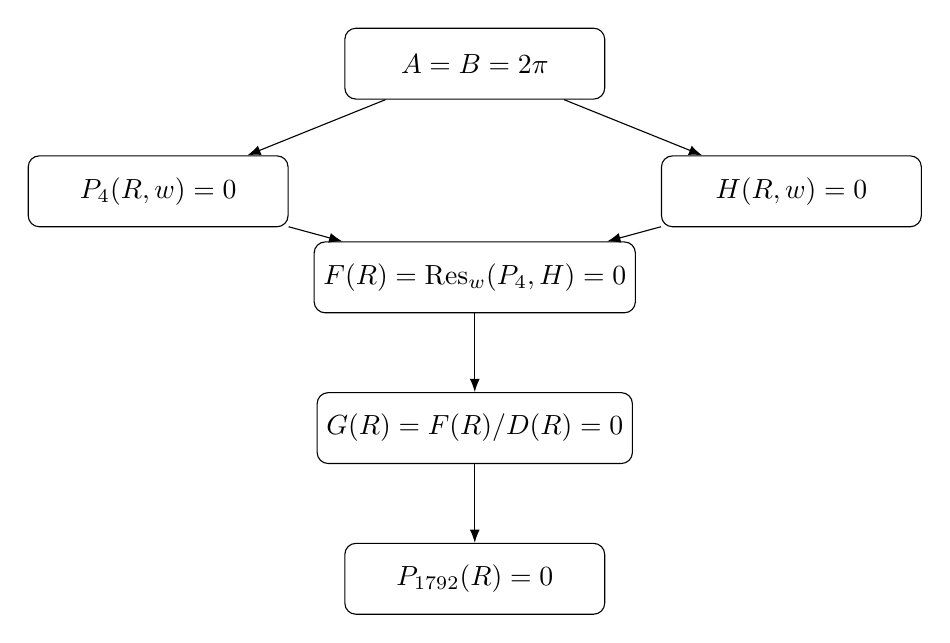
\begin{tikzpicture}[node distance=10mm, >=Latex,
  box/.style={draw, rounded corners, align=center, minimum width=33mm, minimum height=9mm}]
  \node[box] (ab) {$A=B=2\pi$};
  \node[box, below left=of ab] (p4) {$P_4(R,w)=0$};
  \node[box, below right=of ab] (hh) {$H(R,w)=0$};
  \node[box, below=18mm of ab] (res) {$F(R)=\Res_w(P_4,H)=0$};
  \node[box, below=of res] (gg) {$G(R)=F(R)/D(R)=0$};
  \node[box, below=of gg] (pp) {$P_{1792}(R)=0$};
  \draw[->] (ab)--(p4);
  \draw[->] (ab)--(hh);
  \draw[->] (p4)--(res);
  \draw[->] (hh)--(res);
  \draw[->] (res)--(gg);
  \draw[->] (gg)--(pp);
\end{tikzpicture}
\caption{The logical route from the geometric angular system to the rational
norm polynomial.}
\label{fig:flow}
\end{figure}

\section{The exact coefficients of $G$}

Use the radical basis
\[
\begin{aligned}
 (b_0,\ldots,b_{15})={}&(1,\sqrt2,\sqrt3,\sqrt6,\sqrt5,\sqrt{10},\\
 &\sqrt{15},\sqrt{30},\sqrt7,\sqrt{14},\sqrt{21},\sqrt{42},\\
 &\sqrt{35},\sqrt{70},\sqrt{105},\sqrt{210}).
\end{aligned}
\]
Then
\[
 G(R)=\sum_{j=0}^{112}\left(\sum_{m=0}^{15}a_{j,m}b_m\right)R^j,
 \qquad a_{j,m}\in\mathbb{Q}.
\]

\begin{sloppypar}
The complete exact $113\times16$ coefficient array is supplied in
\texttt{circle\_G112\_exact\_coefficients.tsv}; its primitive integer normalization
and
the complete degree--1792 norm coefficient array are supplied in the
reproducibility bundle.  The mathematical definition of $G$ above is
independent of decimal approximations: the table is an exact expansion of
the resultant quotient.  The coefficient-table replay checks all 1808
radical-basis entries modulo an independent prime, and additional prime
checks verify the independent finite-field construction.
\end{sloppypar}

For compactness, the full machine-readable array is not typeset as thousands
of unreadable page-width fractions in the main text.  Its exact location,
normalization, and SHA-256 digest are part of the accompanying certificate
boundary described in Appendix~\ref{app:boundary}.

\section{The algebraic definition of $R_0$}

Let
\[
 P_{1792}(R)=\Norm_{K/\mathbb{Q}}(G(R)),
\]
after monic normalization and primitive integer clearing of denominators.
It is a rational polynomial of degree $16\cdot112=1792$.

\begin{definition}
Let $R_0$ be the unique real root of the primitive integer polynomial
$P_{1792}$ in
\[
 I_0=\bigl[
 8.3034681221114890787043811875161993,
 8.3034681221114890787043811875161994
 \bigr].
\]
\end{definition}

The endpoint signs are checked exactly by evaluating the denominator-cleared
integer polynomial with a rational Horner recurrence.  A certified derivative
or Taylor bound proves uniqueness in $I_0$.  No ordinary floating-point
evaluation is used for this root-isolation claim.

\section{Identification theorem}

\begin{lemma}[Triangle relation]
At a nondegenerate positive-angle solution of $A=B=2\pi$,
\[
 \alpha_5+\beta_{57}-\alpha_7=0.
\]
\end{lemma}
\begin{proof}
Subtract the definitions of $A$ and $B$.  All common chain terms cancel.
\end{proof}

\begin{lemma}[Chain eliminant]
At the same solution, with
\[
 w=\cos(\beta_{79}+\beta_{92}+\beta_{28}+\beta_{86}),
\]
one has $P_4(R,w)=0$.
\end{lemma}
\begin{proof}
Apply the cosine addition identity successively to the four consecutive
angles.  Equation $\Gamma(z;a,b)=0$ is precisely the squared form of that
identity.  The resultant definitions of $P_2,P_3,P_4$ then imply the claim.
\end{proof}

\begin{lemma}[Triangle closure eliminant]
At the same positive-angle contact realization, $H(R,w)=0$.
\end{lemma}
\begin{proof}
The triangle relation from the preceding lemma determines the oriented
$5$--$7$--$10$ triangle.  Substituting its cosine and sine relations into the
$(6,10)$ distance equation and eliminating the remaining sine variables gives
the displayed polynomial $H$.  The argument is only used in the forward
direction, so the squaring steps used to remove radicals introduce no logical
problem.
\end{proof}

\begin{theorem}[Equality of the two radius definitions]
Assume the exact contact-elimination identities above, together with a
certified refinement placing $R_{\mathrm{crit}}$ in $I_0$, and the certified
uniqueness of the $P_{1792}$ root in $I_0$.  Then
\[
 \boxed{R_{\mathrm{crit}}=R_0}.
\]
\end{theorem}
\begin{proof}
The preceding lemmas give a common root $w$ of $P_4(R_{\mathrm{crit}},w)$ and
$H(R_{\mathrm{crit}},w)$.  Hence
\[
F(R_{\mathrm{crit}})=0.
\]
Since $R_{\mathrm{crit}}>8$, no factor of $D(R_{\mathrm{crit}})$ vanishes,
so $G(R_{\mathrm{crit}})=0$.  Taking the field norm gives
\[
P_{1792}(R_{\mathrm{crit}})=0.
\]
The refined interval certificate places $R_{\mathrm{crit}}$ in $I_0$.
The root-isolation certificate says that $P_{1792}$ has exactly one root in
$I_0$, namely $R_0$.  Therefore $R_{\mathrm{crit}}=R_0$.
\end{proof}

\begin{remark}[Certificate status]
The broad interval certificate in Section~4 establishes the geometric root in
$J_R$.  To turn the displayed conditional theorem into a completed equality
certificate, one must additionally replay the refinement
$R_{\mathrm{crit}}\in I_0$ and the exact algebraic implication from the
positive-angle contact equations to $P_4=H=0$.  The theorem is stated with
these hypotheses explicitly rather than treating overlapping decimal
intervals as an equality proof.
\end{remark}

\section{Conclusion and scope}

We have described two definitions of the radius of the selected contact
configuration and the exact elimination bridge between them.  The conclusion
is the identity
\[
 R_{\mathrm{crit}}=R_0.
\]
This note does not claim that no other ten-circle configuration has a smaller
radius.  Proving such a global statement requires a separate exhaustive
geometric coverage theorem.

\appendix
\section{Exact coefficient and certificate data}
\label{app:coefficients}

The full coefficient files are:
\begin{itemize}
\item \texttt{circle\_G112\_exact\_coefficients.tsv}, the exact $K$-basis table for $G$;
\item \texttt{circle\_G112\_primitive\_integer\_coefficients.tsv}, the primitive integer
      normalization;
\item \texttt{data/P1792\_primitive\_integer\_coefficients.tsv}, the complete norm
      polynomial over $\mathbb{Z}$.
\end{itemize}
Their hashes and replay instructions are recorded in the accompanying
README.  These files are data representations of the explicitly defined
resultants, not independent numerical definitions.

\section{External arithmetic and Lean boundary}
\label{app:boundary}

The external layer performs resultants, exact multiquadratic arithmetic,
finite-field checks, coefficient reconstruction, and rational interval
certification.  Lean imports the exact coefficient literals and proves the
downstream logical implications from an explicit contact-elimination bridge.
In particular, Lean can assemble
\[
\text{contact bridge}+P_{1792}\text{ root data}
\Longrightarrow P_{1792}(R_0)=0
\Longrightarrow R_0\text{ is algebraic over }\mathbb{Q}.
\]
The current Lean interface intentionally does not treat a log file, a decimal
approximation, or a SHA-256 hash as a theorem.  Formalizing the large
resultant identities and replacing the bridge assumptions by independently
checked replay theorems remains a separate task.

\section{Reproduction commands}

From the repository root, the exact arithmetic smoke tests can be run with
the bundled scripts.  The Lean coefficient interface can be checked with
\begin{verbatim}
cd lean
lake env lean CirclePacking/P1792.lean
\end{verbatim}

\end{document}
